\PassOptionsToPackage{disable}{endfloat}
\documentclass[floatsintext, stu, 12pt]{apa7}
\usepackage{mathptmx}
\usepackage{amsmath}
\usepackage[spanish,mexico]{babel}
\usepackage{bookmark}
\usepackage[style=apa]{biblatex}
\usepackage{csquotes}
\usepackage{longtable}
\usepackage{booktabs}
\usepackage{tabularx}
\usepackage{graphicx}
\usepackage{geometry}
\usepackage{caption}
\usepackage{subcaption}
\usepackage{array}
\usepackage{float}
\usepackage{setspace}
\usepackage{hyperref}
\floatplacement{figure}{H}
\floatplacement{table}{H}
% --- Configuración de captions estilo APA 7 ---
\captionsetup{
	justification=justified,
	singlelinecheck=false,
	labelfont=bf,
	labelsep=period
}
% Configuración específica para las sub-figuras
\captionsetup[subfigure]{
	labelfont=rm, % Letra normal para (a), (b)
	labelformat=simple % Formato simple (a, b)
}
\geometry{letterpaper, margin=2.5cm}
\setlength{\parindent}{2em}
\setlength{\parskip}{0pt}
\graphicspath{{images/}}

\addbibresource{references.bib}
\hypersetup{
	colorlinks=true,
	urlcolor=blue,
	linkcolor=black
}

\newcolumntype{L}{>{\raggedright\arraybackslash}X}

\title{Red de edificio de Aulas}
\authorsnames{Cárdenas Camacho Alexis \textendash{} 295592, Juárez Ramírez Gabriel \textendash{} 325846, Macías Fonseca Alejandro \textendash{} 325724, Mata Guerra David \textendash{} 325797}
\authorsaffiliations{Facultad de Informática, Universidad Autónoma de Querétaro}
\course{Diseño y Soporte de Redes}
\professor{Mtro. Ing. César Estévez Serrato}
\duedate{28 de noviembre de 2025}

\begin{document}
\setstretch{2.0}
\maketitle
\tableofcontents
\clearpage
\input{planificacion-design/planificacion-design.tex}
\input{configuracion/implementacion-red.tex}
\input{monitoreo-analisis/monitoreo-analisis.tex}
\section{Implementación de Seguridad}
\input{implementacion-seguridad/politicas-seguridad.tex}
\subsection{Solución de Firewall (Hardware y Software)}
Los firewalls constituyen un componente esencial en la seguridad de redes moderna. Actúan como una barrera de defensa fundamental, cuya función principal es supervisar, filtrar y controlar todo el tráfico de red entrante y saliente basándose en un conjunto de reglas de seguridad predefinidas. Su objetivo es identificar y bloquear el tráfico no deseado o malicioso antes de que pueda comprometer los activos internos. De esta manera, los firewalls se convierten en una de las herramientas de protección de información con mayor relevancia, ayudando a preservar los tres pilares de la seguridad de la información: la integridad, la confidencialidad y la disponibilidad \parencite{MoraBandera2020}

La solución propuesta se compone de una plataforma de hardware dedicada y un sistema operativo de firewall de nueva generación.

\subsubsection{Plataforma de Hardware}
El hardware seleccionado es el \textbf{Fortinet FortiGate 60F}. Este equipo es un firewall físico de nueva generación (NGFW) diseñado para redes empresariales pequeñas y medianas, con mayor capacidad de procesamiento y seguridad avanzada que modelos de entrada.

La justificación de esta elección se basa en varios puntos clave:
\begin{itemize}
    \item \textbf{Rendimiento de Red:} Ofrece un throughput de firewall superior a 10 Gbps y protección contra amenazas adecuada para el tráfico de un edificio de aulas con múltiples VLAN, usuarios concurrentes y crecimiento futuro.
    \item \textbf{Segmentación y VLANs Dinámicas:} Soporta múltiples VLAN y permite, mediante 802.1X/RADIUS, asignar dinámicamente la VLAN según el usuario o dispositivo, lo que facilita separar tráfico de administración, profesores, alumnos, cámaras y VoIP.
    \item \textbf{Seguridad Avanzada:} Integra capacidades de inspección profunda de paquetes, IPS, filtrado web, control de aplicaciones y antivirus, alineadas con el modelo de seguridad de próxima generación.
    \item \textbf{VPN y Acceso Remoto:} Permite crear túneles VPN IPsec y SSL para acceso seguro de profesores y personal administrativo a los recursos internos.
    \item \textbf{Gestión Centralizada:} Puede administrarse mediante su interfaz web o integrarse a plataformas de gestión como FortiCloud o FortiManager para monitoreo centralizado.
    \item \textbf{Costo y Soporte:} El modelo FortiGate 60F se mantiene dentro del presupuesto asignado (aproximadamente \$13,899 MXN) y se complementa con la licencia de soporte FortiCare Premium de 1 a\~no, lo que asegura actualizaciones y acompañamiento del fabricante.
\end{itemize}

\subsubsection{Plataforma de Software (NGFW)}
El FortiGate 60F opera con \textbf{FortiOS}, el sistema operativo propietario de Fortinet para firewalls de nueva generación. FortiOS proporciona una interfaz gráfica moderna para la administración del firewall, la configuración de servicios de red (DHCP, DNS), la creación de VPNs y el monitoreo detallado del tráfico y de los eventos de seguridad.

La justificación para la elección de FortiOS complementa al hardware:
\begin{itemize}
    \item \textbf{Capacidades NGFW Integradas:} Incluye inspección con estado, IPS, filtrado web, control de aplicaciones y protección frente a amenazas avanzadas como parte de la plataforma de seguridad.
    \item \textbf{Gestión y Visibilidad:} La interfaz de administración permite definir políticas por VLAN, subred o usuario, así como visualizar sesiones activas, estadísticas de tráfico y eventos de seguridad en tiempo real.
    \item \textbf{Actualizaciones y Soporte:} Junto con la suscripción FortiCare Premium (1 año), se obtiene acceso a actualizaciones de firmware, soporte técnico y actualizaciones de firmas de seguridad.
\end{itemize}
\subsection{Buenas Prácticas de Seguridad}

Para mantener el entorno seguro con medidas concretas y breves:

\begin{itemize}
    \item \textbf{Antimalware en equipos conectados:} motor actualizado, análisis programados.
    \item \textbf{Cifrado en tránsito:} usar TLS 1.2 basado en AES-256; en WiFi, WPA3. 
    \item \textbf{Cifrado en reposo:} proteger respaldos y dispositivos críticos con AES-256; gestionar llaves en un almacén seguro con rotación periódica.
    \item \textbf{VPN institucional:} todo acceso remoto debe ir por la VPN. Aplicar mínimo privilegio y dar de baja credenciales inactivas.
    \item \textbf{Acceso a cuartos de racks:} control físico con cerraduras electrónicas y autenticación biométrica preferente, registro de entradas y política de visitantes.
    \item \textbf{Control de acceso lógico:} mínimo privilegio, cuentas nominales y una robusta auditoría periódica.
    \item \textbf{IDS/IPS:} desplegar en segmentos críticos, con firmas actualizadas y revisión de alertas.
\end{itemize}

\subsection{Herramientas de seguridad adicionales}\label{sec:herramientas-adicionales}

WireGuard es un túnel VPN moderno orientado al rendimiento y la simplicidad operativa. Utiliza criptografía actual, opera sobre UDP, y se integra con facilidad en entornos de campus y acceso remoto. Para su implementación se recomienda: generar pares de claves por dispositivo, definir pares (\textit{peers}) con \texttt{AllowedIPs} específicos, publicar el servicio en el puerto UDP 51820, aplicar reglas de cortafuegos que restrinjan el alcance de las subredes expuestas y habilitar registro de eventos para auditoría.

\begin{figure}[H]
	\centering
	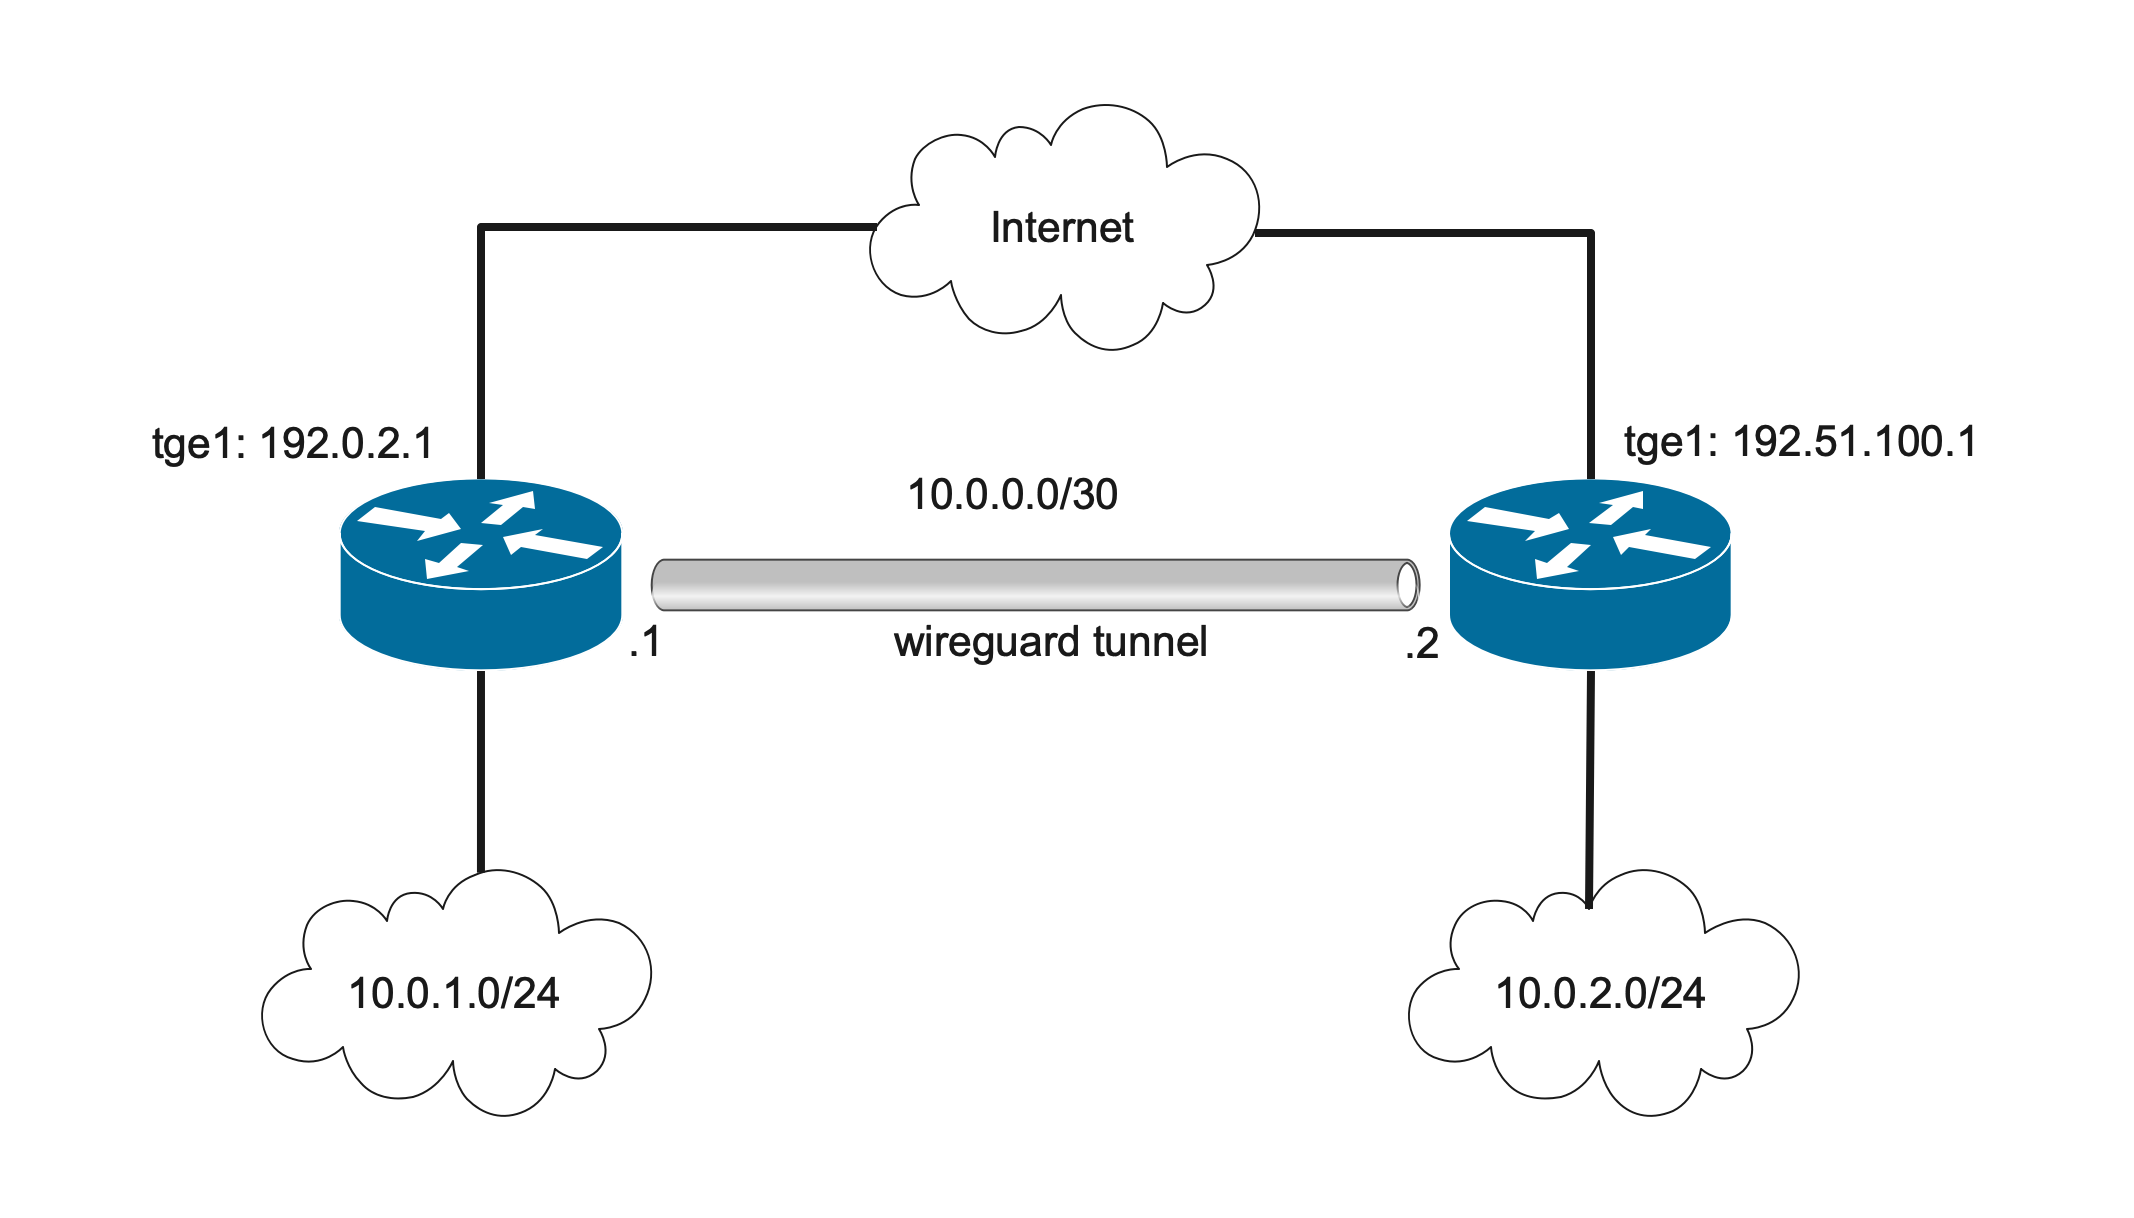
\includegraphics[width=0.9\linewidth]{images/wireguard-example}
	\caption{Ejemplo de topología con WireGuard}\label{fig:wireguard-example}
\end{figure}



Como complemento a la VPN, se sugieren herramientas puntuales para refuerzo defensivo:

- \textit{Suricata} (IDS/IPS): motor de inspección profunda de paquetes que permite detección y prevención de intrusiones, útil en modo espejo (IDS) o en línea (IPS) con reglas actualizadas. Facilita visibilidad sobre patrones anómalos y ataques comunes. 

- \textit{Wazuh} (Antimalware): plataforma de seguridad y monitoreo que integra capacidades de detección de malware, análisis de integridad y gestión de vulnerabilidades. Permite la supervisión continua de endpoints y servidores, generando alertas ante actividades sospechosas. Su arquitectura distribuida facilita la escalabilidad en entornos de red complejos.

\begin{figure}[H]
	\centering
	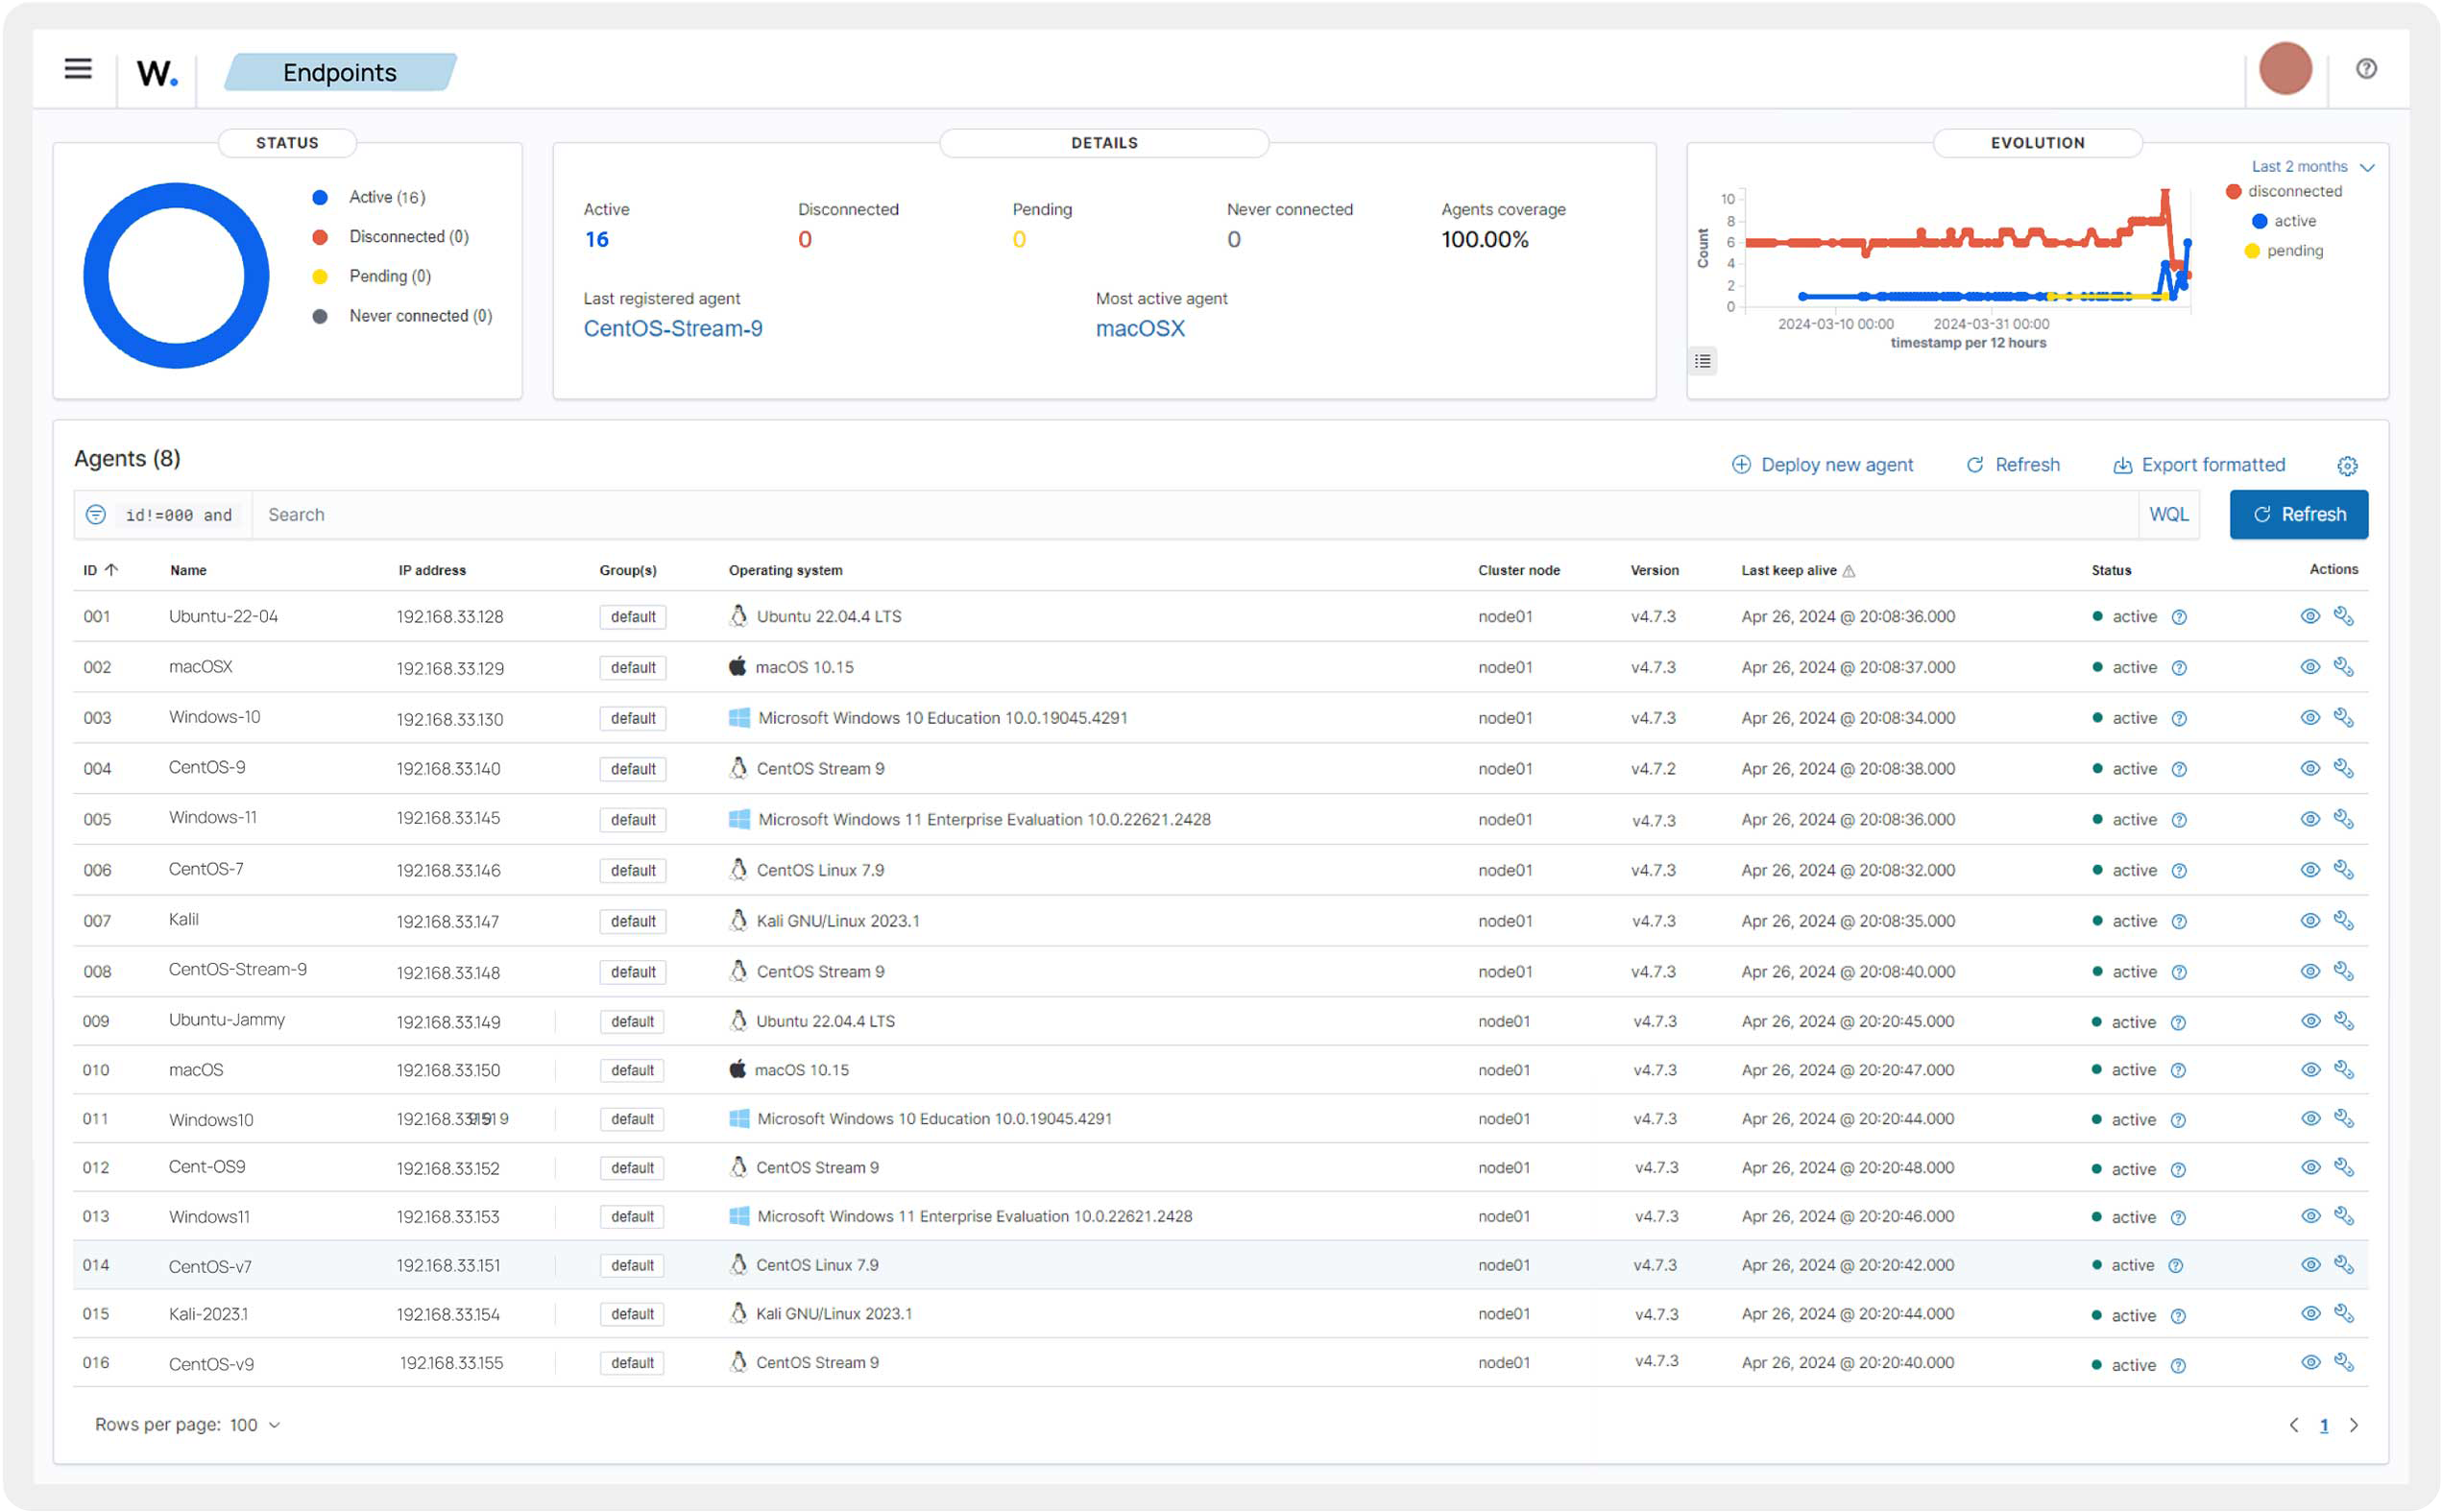
\includegraphics[width=0.9\linewidth]{images/wazuh}
	\caption{Vista referencial de Wazuh}\label{fig:wazuh}
\end{figure}


\input{implementacion-seguridad/consideraciones.tex}


\subsection{Descripción del Servicio}

El presente Acuerdo de Nivel de Servicio (SLA) establece las condiciones bajo las cuales se proporciona el servicio de conectividad y soporte de red al edificio de aulas de la Facultad de Informática. El objetivo principal del servicio es garantizar que estudiantes, docentes y personal administrativo cuenten con acceso disponible, seguro y confiable a los recursos de comunicación y a Internet necesarios para el desarrollo de sus actividades académicas y operativas.

El servicio contratado incluye la provisión y operación de la infraestructura de red del edificio, la atención de incidentes y solicitudes relacionados con la conectividad, el monitoreo básico del estado del servicio y la aplicación de las políticas de seguridad definidas por la institución. Todos estos elementos se prestan de acuerdo con los niveles de disponibilidad, tiempos de respuesta y alcances que se describen en las secciones posteriores de este SLA.

El servicio de red incluye:
\begin{itemize}
    \item Conectividad a la red cableada entre el edificio de aulas y edificio de Innovaci\'on.
    \item Conectividad a la red inalámbrica (Wi-Fi) al alcance de todas las aulas.
    \item Acceso a Internet de alta velocidad.
    \item Soporte técnico para la resolución de problemas relacionados con la conectividad de red.
\end{itemize}

\subsection{Alcance de Acuerdos}

Este SLA se aplica a todos los usuarios de la red del edificio de aulas, incluyendo estudiantes, profesores y personal administrativo. El acuerdo cubre la disponibilidad, rendimiento y soporte de los servicios de red descritos en la sección anterior.

\subsubsection{Disponibilidad del Servicio}
El objetivo es mantener una disponibilidad de la red del 99.5\% durante el horario de servicio establecido. La disponibilidad se medirá mensualmente y se calculará como el porcentaje de tiempo en que los servicios de red estuvieron operativos y accesibles.

\subsubsection{Rendimiento de la Red}
La red se diseñará y mantendrá para proporcionar un rendimiento adecuado para las actividades académicas y administrativas. Esto incluye un ancho de banda suficiente para la navegación web, el acceso a recursos en línea, la transmisión de video y otras aplicaciones de uso común.

\subsubsection{Soporte Técnico}
El soporte técnico se proporcionará a través de los canales de comunicación y en el horario establecido en este acuerdo. El objetivo es responder a las solicitudes de soporte de manera oportuna y resolver los problemas de red de manera eficiente.

\subsection{Contactos}

Para cualquier consulta o problema relacionado con el servicio cubierto por este SLA, se establecen los siguientes contactos de soporte organizados por niveles de atención:

\subsubsection*{Nivel 1 \\ Mesa de Ayuda de Aulas}
\begin{itemize}
	\item \textbf{Nombre:} Ing. David Mata Guerra\\
    	\textbf{Puesto:} Analista de Soporte de Primer Nivel (Mesa de Ayuda)\\
    	\textbf{Correo:} \href{mailto:mesa.ayuda.aulas@universidad.edu}{mesa.ayuda.aulas@universidad.edu}\\
    	\textbf{Teléfono:} +52 (442) 192 1200 Ext. 3101
\end{itemize}

Responsable de recibir y registrar todos los reportes de fallas y solicitudes de servicio, realizar el diagnóstico inicial y resolver incidentes básicos relacionados con conectividad de usuario, autenticación y acceso a recursos.

\subsubsection*{Nivel 2 \\ Soporte Especializado de Redes}
\begin{itemize}
	\item \textbf{Nombre:} Mtro. Gabriel Juárez Ramírez\\
    	\textbf{Puesto:} Ingeniero de Redes Campus Aulas\\
    	\textbf{Correo:} \href{mailto:soporte.redes.aulas@universidad.edu}{soporte.redes.aulas@universidad.edu}\\
    	\textbf{Teléfono:} +52 (442) 192 1200 Ext. 3205
\end{itemize}

Encargado de atender incidentes escalados desde el Nivel 1 que involucren equipo de conmutación, enlaces troncales, VLANs, puntos de acceso inalámbricos o configuración del firewall perimetral.

\subsubsection*{Nivel 3 \\ Coordinación de Infraestructura y Escalamiento a Proveedores}
\begin{itemize}
	\item \textbf{Nombre:} Mtro. Alejandro Macías Fonseca\\
    	\textbf{Puesto:} Coordinador de Infraestructura de Redes\\
    	\textbf{Correo:} \href{mailto:infraestructura.redes@universidad.edu}{infraestructura.redes@universidad.edu}\\
    	\textbf{Teléfono:} +52 (442) 192 1200 Ext. 3302
\end{itemize}

Responsable de la gestión de incidentes críticos, decisiones de cambio mayor, coordinación con el proveedor de servicios de Internet y con fabricantes (por ejemplo, soporte de Fortinet o Aruba) cuando se requiera soporte de tercer nivel.\\[0.5em]

Como contacto alterno de nivel ejecutivo se designa a \textbf{Alexis Emilio Cárdenas Camacho}, responsable de supervisar el cumplimiento general del SLA y aprobar acciones extraordinarias cuando sea necesario.

\subsubsection*{Canales Generales de Atención}
Además de los contactos anteriores, se disponen los siguientes canales generales para el registro y seguimiento de casos:
\begin{itemize}
    \item \textbf{Portal de Soporte en Línea:} \url{https://soporte.universidad.edu/redes}
    \item \textbf{Teléfono de la Mesa de Ayuda:} +52 (442) 192 1200 Ext. 3100
\end{itemize}

El flujo de escalamiento se inicia siempre en el Nivel 1 y progresa a los niveles superiores únicamente cuando el incidente no pueda ser resuelto en el nivel previo o cuando, por su impacto, sea clasificado como incidente mayor según lo definido en este SLA.

\subsection{Horario del Servicio}

El servicio de soporte definido en este SLA se presta principalmente en horario hábil académico, durante el cual se garantiza la atención de incidentes y solicitudes según los tiempos de respuesta establecidos.

\begin{itemize}
    \item \textbf{Lunes a Viernes (Soporte Completo):} de 7:00 a 22:00 horas.
    \item \textbf{Sábados (Soporte Reducido):} de 8:00 a 14:00 horas.
\end{itemize}

Fuera de este horario, la infraestructura de red permanece operando de manera continua, pero la atención de soporte se limita a incidentes críticos que afecten a todo el edificio y estará sujeta a la disponibilidad del personal de guardia. Las solicitudes no críticas registradas fuera del horario de servicio se atenderán al siguiente día hábil.

\subsection{Escalamiento}

El proceso de escalamiento garantiza que las incidencias relacionadas con el servicio de red sean atendidas de manera oportuna y por el nivel de soporte adecuado, de acuerdo con la estructura de contactos definida en este SLA.

\subsubsection*{Niveles de Escalamiento}
\begin{itemize}
    \item \textbf{Nivel 1: Mesa de Ayuda de Aulas.} Primer punto de contacto para el registro de incidentes y solicitudes. Realiza el diagnóstico inicial, aplica soluciones estándar y da seguimiento básico. Si el incidente no puede ser resuelto o se detecta que afecta a múltiples usuarios o servicios críticos, se escalara al Nivel 2 con toda la información recolectada (descripción, impacto, bitácora de acciones y evidencias).
    \item \textbf{Nivel 2: Soporte Especializado de Redes.} Atiende incidentes escalados desde el Nivel 1 que involucren conmutadores, enlaces troncales, VLANs, Wi-Fi o firewall perimetral. Si el incidente presenta impacto crítico (por ejemplo, indisponibilidad total del edificio o riesgo de seguridad), o requiere cambios mayores en la infraestructura, el caso se escalara al Nivel 3.
    \item \textbf{Nivel 3: Coordinación de Infraestructura y Proveedores.} Responsable de la gestión de incidentes mayores, coordinación de cambios significativos, relación con el proveedor de Internet y fabricantes, así como de la toma de decisiones para la restauración del servicio cuando se requieran acciones extraordinarias.
\end{itemize}

En cada cambio de nivel, se actualiza el estado del incidente en la bitácora correspondiente y se notifica a la parte contratante sobre el progreso y las acciones en curso.

\subsubsection*{Clasificación de Incidencias y Tiempos de Atención}
Las incidencias se clasifican según su impacto y urgencia, definiendo tiempos objetivo de respuesta (inicio de la atención) y de resolución (restauración del servicio o aplicación de una solución temporal aceptable). La Tabla~\ref{tab:escalamiento-incidencias} resume estos parámetros.

\begin{table}[H]
    \centering
    \caption{Clasificación de incidencias y tiempos de atención}\label{tab:escalamiento-incidencias}
    \begin{tabular}{p{4cm}p{5cm}cc}
        	\toprule
        	\textbf{Clasificación} & \textbf{Descripción} & \textbf{Tiempo de respuesta} & \textbf{Tiempo de resolución} \\
        \midrule
        Crítica & Caída total del servicio de red en el edificio o incidente de seguridad grave. & Hasta 2 hora & Hasta 4 horas \\
        Alta & Afectación parcial significativa (varias aulas o servicios clave). & Hasta 2 horas & Hasta 8 horas \\
        Media & Problemas que afectan a un conjunto reducido de usuarios o servicios no críticos. & Hasta 2 horas & Hasta 24 horas \\
        Baja & Solicitudes de servicio, dudas o mejoras sin impacto directo en la disponibilidad. & Hasta 2 día hábil & Hasta 5 días hábiles \\
        \bottomrule
    \end{tabular}
\end{table}

\subsection{Reportes}

Se generarán los siguientes reportes para monitorear el cumplimiento de este SLA:

\begin{itemize}
    \item \textbf{Reporte Mensual de Disponibilidad:} Este reporte mostrará el porcentaje de disponibilidad de la red durante el mes, así como los incidentes que causaron interrupciones en el servicio.
    \item \textbf{Reporte Mensual de Rendimiento:} Se incluirán métricas de rendimiento de la red, como el ancho de banda utilizado, la latencia y la pérdida de paquetes.
    \item \textbf{Reporte Mensual de Soporte Técnico:} Se presentará un resumen de las solicitudes de soporte recibidas, los tiempos de respuesta y los tiempos de resolución.
\end{itemize}

Estos reportes se enviarán a la dirección de la Facultad de Informática y estarán disponibles para su consulta en el portal de soporte en línea.

\section{Responsabilidades, Limitaciones y Restricciones}

\subsection{Responsabilidades del Proveedor del Servicio}
\begin{itemize}
    \item Mantener la infraestructura de red en óptimas condiciones.
    \item Monitorear la red para detectar y resolver problemas de manera proactiva.
    \item Proporcionar soporte técnico de acuerdo a lo establecido en este SLA.
    \item Notificar a los usuarios sobre mantenimientos programados que puedan afectar el servicio.
\end{itemize}

\subsection{Responsabilidades de los Usuarios}
\begin{itemize}
    \item Utilizar la red de manera responsable y de acuerdo a las políticas de la universidad.
    \item No realizar actividades que puedan comprometer la seguridad o el rendimiento de la red.
    \item Reportar cualquier problema de red a través de los canales de comunicación establecidos.
    \item Proporcionar información clara y precisa al solicitar soporte técnico.
\end{itemize}

\subsection{Limitaciones y Restricciones}
\begin{itemize}
    \item El proveedor del servicio no se hace responsable por problemas causados por el mal uso de la red por parte de los usuarios.
    \item La disponibilidad del servicio puede verse afectada por factores fuera del control del proveedor, como cortes de energía eléctrica o fallas en el proveedor de servicios de Internet.
    \item Se podrán aplicar restricciones de ancho de banda a ciertos servicios o aplicaciones para garantizar un rendimiento equitativo para todos los usuarios.
\end{itemize}

\subsection{Costos}

El servicio de red se proporciona sin costo directo para los estudiantes, profesores y personal administrativo de la Facultad de Informática, ya que está cubierto por el presupuesto operativo de la universidad.

Sin embargo, se podrán aplicar cargos adicionales en los siguientes casos:
\begin{itemize}
    \item Solicitudes de servicios de red especializados que no formen parte de la oferta estándar.
    \item Daños a la infraestructura de red causados por negligencia o mal uso por parte de un usuario.
\end{itemize}

Cualquier cargo adicional se notificará y acordará con el solicitante antes de realizar cualquier trabajo.

\section{Metodología de Respuesta a Fallas}

Para garantizar una respuesta rápida y efectiva a las fallas de la red, se seguirá la siguiente metodología basada en el ciclo de vida de la gestión de incidentes:

\begin{enumerate}
    \item \textbf{Detección y Registro:} Las fallas pueden ser detectadas por el sistema de monitoreo proactivo o reportadas por los usuarios. En ambos casos, se registrará un ticket en el sistema de soporte con toda la información relevante.
    \item \textbf{Clasificación y Priorización:} Cada incidente se clasificará según su impacto (número de usuarios afectados) y urgencia (criticidad de los servicios afectados). Esto determinará la prioridad para su atención.
    \begin{itemize}
        \item \textbf{Prioridad Alta:} Falla general de la red, afectando a un gran número de usuarios o servicios críticos.
        \item \textbf{Prioridad Media:} Falla parcial que afecta a un grupo de usuarios o a un servicio no crítico.
        \item \textbf{Prioridad Baja:} Problema de conectividad de un solo usuario o degradación menor del servicio.
    \end{itemize}
    \item \textbf{Diagnóstico y Solución:} El equipo de soporte técnico investigará la causa raíz del problema. Una vez identificada, se aplicará la solución correspondiente, que puede ir desde un reinicio de equipo hasta una reconfiguración de la red.
    \item \textbf{Recuperación y Cierre:} Después de aplicar la solución, se verificará que el servicio se haya restablecido por completo y que el problema esté resuelto. Se documentará la solución en el ticket y se procederá a su cierre, notificando al usuario.
    \item \textbf{Análisis Post-Incidente:} Para incidentes de alta prioridad, se realizará un análisis posterior para identificar la causa fundamental y definir acciones preventivas que eviten su recurrencia en el futuro.
\end{enumerate}

\subsection{Seguimiento y Control de Fallas}

El seguimiento y control de todas las fallas reportadas se gestionará de manera centralizada para asegurar una resolución transparente y eficiente.

\subsubsection{Sistema de Tickets}
Se utilizará un sistema de gestión de tickets (por ejemplo, OTRS, Jira Service Management o similar) como herramienta principal para el registro, seguimiento y control de todas las incidencias. Cada vez que se reporte una falla, se creará un ticket único con un número de identificación. Este ticket contendrá toda la información relevante del incidente, incluyendo:
\begin{itemize}
    \item Descripción del problema.
    \item Fecha y hora del reporte.
    \item Usuario que reporta.
    \item Nivel de prioridad asignado.
    \item Técnico asignado.
    \item Todas las acciones y comunicaciones realizadas.
    \item Solución final y fecha de cierre.
\end{itemize}

\subsubsection{Comunicación y Notificaciones}
El usuario que reportó la falla recibirá notificaciones automáticas por correo electrónico en cada etapa clave del proceso:
\begin{itemize}
    \item Creación del ticket.
    \item Asignación de un técnico.
    \item Actualizaciones importantes sobre el progreso.
    \item Cierre del ticket.
\end{itemize}
Además, los usuarios podrán consultar el estado de sus tickets en cualquier momento a través del portal de soporte en línea, utilizando el número de identificación de su ticket.

\subsubsection{Monitoreo del Cumplimiento}
El administrador de la red revisará periódicamente los tickets abiertos y cerrados para supervisar el cumplimiento de los tiempos de respuesta y solución establecidos en este SLA. Los resultados de este monitoreo se incluirán en los reportes mensuales de soporte técnico.


\printbibliography%
\end{document}
